\chapter{实验介绍}
为了比较合肥市城市与郊区能量以及其它气象要素的差异,
使用了中科大站(USTC)和科学岛站(HFCAS)两气象观测站的观测数据,
它们的地理位置如图\ref{fig:map},
中科大站的观测设备位于合肥市金寨路 96 号中国科学技术大学东区第一教学楼楼顶,
地处市中心附近,中科大站的观测塔共三层
科学岛站的五层气象观测塔设在庐阳区科学岛大气成分与光学重点实验室一处开阔草坪上,
它位于郊区且在董铺水库水边。
两座铁塔可观测温度、气压、湿度、风速、风向、辐射、二氧化碳、水汽等气象要素。
\begin{figure}[H]
\centering
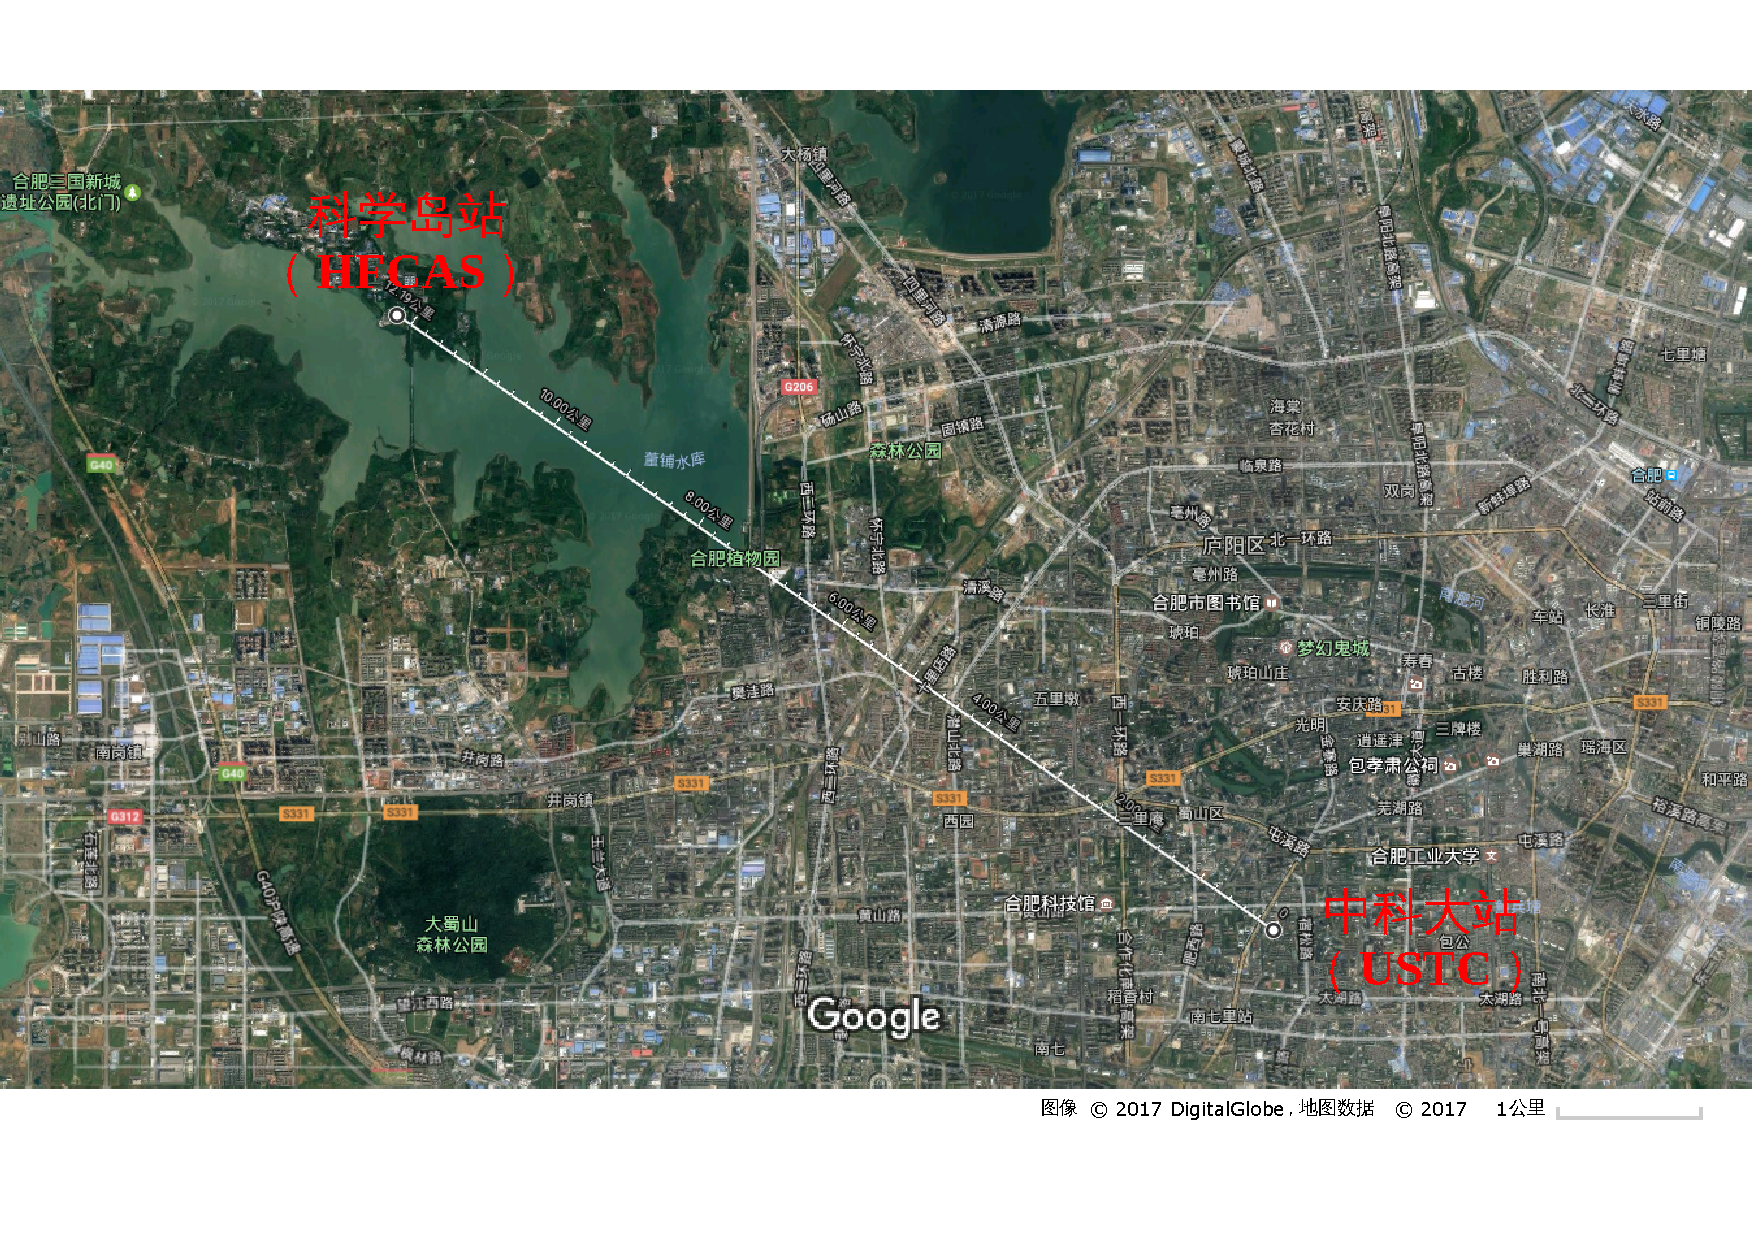
\includegraphics[width=.9\linewidth]{map}
\caption{中科大站(USTC)与科学岛站(HFCAS)的地理位置}\label{fig:map}
\note{图片来自 Google 地图}
\end{figure}

科大站的气象观测塔由 1 台 EC50 涡动相关系统(CSAT3A 三维超声风速仪头和 EC150 开路分析仪),
1 个 CNR4 净辐射表,3 个 HMP155A 空气温湿度,
3 个 03002 风速风向传感器, 1 台 CR3000 数据采集器,及其他备件组成。
EC150 开路分析仪作为涡动相关系统的一部分,其本身也可测量二氧化碳和水汽的浓度、大气温度以及气压,
配合 CSAT3A 使用还可测量三维风速和超声大气温度。
CNR4 由两对辐射测量仪组成,一对可测向下向上的短波辐射通量密度(DSR,USR),
另一对可测向下向上的长波辐射通量密度(DLR,ULR),
向下辐射与向上辐射做差可得净辐射通量密度(Rn)。观测塔每层设有一个 HMP155A 空气湿度温度传感器,
一个 03002 风速风向传感器,HMP155A 用来测量相对湿度(RH)和大气温度(Ta),
03002 由风杯和风向标组成用来测量各层的风速风向。
数据采集箱位于距塔脚 10 米处,各传感器均引线连接到 CR3000 数据采集器,
CR3000 将各传感器获取的气象数据存入存储器中。科学岛站的气象观测塔与科大站的类似不再赘述。
